\documentclass[a4paper,12pt]{article}

% --- Paquetes básicos ---
\usepackage[utf8]{inputenc}
\usepackage[spanish]{babel}
\usepackage{hyperref}
\usepackage{booktabs}
\usepackage{amsmath, amsfonts, amssymb}
\usepackage{listings}
\usepackage{graphicx}
\usepackage{subcaption}
\usepackage{tcolorbox}
\usepackage{enumitem}
\usepackage[a4paper, top=2cm, bottom=2.5cm, left=2.5cm, right=2.5cm]{geometry}
\usepackage{csquotes}
\usepackage[style=ieee, backend=biber]{biblatex}
\addbibresource{references.bib}


\title{\Huge \textbf{Práctica 2: Clasificación de Transacciones mediante PLN}}
\author{Diego Esclarín \and Sofía Contreras}
\date{\today}

\begin{document}

\begin{titlepage}
    \maketitle

    \begin{figure}[h]
        \centering
        \includegraphics[width=0.6\textwidth]{figures/logo_urjc.png}
        \label{fig:logo}
    \end{figure}
    
    \vfill
    \centering
    \large
    Aplicaciones de Inteligencia Artificial \\
    Grado en Ingeniería en Inteligencia Artificial \\
    Universidad Rey Juan Carlos \\
    Curso 2025--26
\end{titlepage}


\newpage
\tableofcontents
\newpage

\section{Introducción}
\label{sec:introduccion}

El propósito fundamental de este proyecto es el desarrollo de una solución inteligente basada en Procesamiento de Lenguaje Natural (PLN) para automatizar uno de los procesos más tediosos en la gestión financiera: la clasificación de movimientos bancarios. En un entorno digital donde el volumen de transacciones personales crece exponencialmente, la capacidad de organizar automáticamente estos datos deja de ser un lujo para convertirse en una necesidad técnica. El sistema diseñado actúa como un puente entre la información desestructurada que emiten las entidades bancarias y la estructura organizada que requiere un usuario para comprender sus hábitos de gasto.

El núcleo de la investigación se centra en la capacidad de interpretación semántica. A diferencia de los sistemas tradicionales basados en reglas rígidas o búsqueda de palabras clave —que suelen fallar ante variaciones ortográficas o sinónimos—, este sistema se enfoca en comprender la intención detrás de cada descripción. Para lograr esta robustez, el proceso de entrenamiento utiliza un corpus de datos diseñado para cubrir un amplio espectro de posibilidades lingüísticas. Se busca que el modelo no solo reconozca términos aislados, sino que sea capaz de gestionar la variabilidad con la que una misma operación financiera puede ser registrada, garantizando así una categorización coherente y precisa en escenarios de uso real.

Finalmente, el proyecto destaca por su capacidad de mejora personalizada. El sistema no es una herramienta estática, sino que permite integrar las correcciones y las nuevas descripciones que el usuario genere en su día a día. Al reentrenar el modelo con estos datos específicos, el clasificador deja de ser una solución generalista para adaptarse al vocabulario y a los hábitos de gasto particulares de cada persona. De esta forma, el sistema garantiza una precisión creciente, optimizando su rendimiento a medida que se acumula un historial de transacciones real y verificado por el propio usuario.
\section{Contexto}
\label{sec:contexto}

El problema abordado es la ineficiencia de indicar manualmente la categoría de gasto de una transacción bancaria. Además de muchas de estas transacciones se repiten recurrentemente, lo que hace que sea una tarea tediosa para el usuario y pueda generar bajas en el uso de la aplicación. 

La heterogeneidad en las descripciones de las transacciones, sumada al volumen de movimientos, impide el uso de reglas fijas o filtros de texto simples, que fallan ante cualquier cambio en la redacción. Por ello, es necesario un sistema basado en Procesamiento de Lenguaje Natural (PLN) más complejo que recoja algo más de información y correlacione para clasificarlas automáticamente en categorías específicas (\textit{Area}). 

Para validar la eficacia de esta clasificación, se utilizan las siguientes métricas:

\begin{itemize}
    \item \textbf{Accuracy (Exactitud):} Mide el porcentaje total de transacciones que el modelo ha clasificado en la categoría correcta.
    \item \textbf{F1-Score:} Evalúa el equilibrio entre la precisión y la capacidad de recuperación del modelo. Es fundamental para asegurar que el sistema clasifique bien tanto las categorías muy comunes (como \textit{Food}) como aquellas con menos ejemplos en el dataset.
\end{itemize}

El objetivo es transformar este flujo de descripciones heterogéneas en información organizada y etiquetada de forma automática.

\newpage
\section{Estado del arte}
\label{sec:estado_arte}

La clasificación de textos financieros ha evolucionado desde sistemas basados en reglas hacia modelos de aprendizaje automático capaces de gestionar la ambigüedad del lenguaje natural.

\begin{itemize}
    \item \textbf{Técnicas de vectorización:} Para transformar texto en datos numéricos, destaca el uso de \textit{TF-IDF}, que asigna pesos a los términos según su relevancia en el corpus, y los \textit{Word Embeddings}, que permiten capturar relaciones semánticas complejas al representar palabras en espacios vectoriales continuos \cite{Minaee2021}.
    
    \item \textbf{Modelos de clasificación:} El uso de algoritmos clásicos como \textit{SVM} y \textit{Random Forest} sigue siendo fundamental en entornos que requieren eficiencia computacional y robustez en textos cortos. Estudios recientes de 2025 confirman que estos modelos ofrecen una mayor consistencia en la clasificación de etiquetas específicas frente a arquitecturas más pesadas \cite{John2025}. Aunque los \textit{Transformers} marcan el estado del arte en precisión, su alta demanda de recursos plantea desafíos de escalabilidad en aplicaciones ligeras \cite{Minaee2021}.
    
    \item \textbf{Aprendizaje incremental (Online Learning):} En el sector financiero, es crucial que los modelos se adapten a nuevos patrones de gasto sin reentrenamientos completos. La automatización de estos procesos requiere algoritmos optimizados (como SGD) que permitan un aprendizaje continuo y eficiente para garantizar la escalabilidad en sistemas de producción \cite{Oyewole2024, Kolluri2019}.
\end{itemize}

\newpage
\section{Propuesta de solución}
\label{sec:propuesta}

Para abordar la clasificación de transacciones financieras, se ha desarrollado un pipeline modular que abarca desde el preprocesamiento de texto hasta la evaluación de múltiples modelos de aprendizaje supervisado.

\subsection{Dataset Unificado y Preprocesamiento}
Después de hacer tests con el dataset original, nos dimos cuenta de que no era suficiente para entrenar un modelo de machine learning, por lo que decidimos combinarlo con el dataset modificado. Aun así, al ser datasets tan diferentes, no evaluaban corréctamente el resto de categorías, por lo que decidimos quedarnos solo con el dataset modificado.

Se han combinado dos fuentes de datos principales: \texttt{db\_orig.csv} y \newline \texttt{db\_modified\_descriptions.csv}, creando un corpus robusto con el doble de ejemplos por categoría y que ha funcionado mejor. Pero la diferencia era demasiado grande y aunque ajustaba mejor decidimos supervisar y depurar la creación de descripciones creando la base de datos \texttt{db\_mod\_descript.csv} que ha mejorado aún más las predicciones. Recordando la importancia que se habló en la primera práctica sobre la gran importancia de la creación y depuración de datos en los problemas que estamos afrontando.
\newline El preprocesamiento incluye:
\begin{itemize}
    \item Conversión a minúsculas y eliminación de caracteres especiales.
    \item Vectorización de texto mediante \textbf{TF-IDF} (\textit{Term Frequency - Inverse Document Frequency}) para transformar las descripciones en representaciones numéricas.
\end{itemize}

\subsection{Comparativa de Modelos}
Se evaluaron cuatro arquitecturas distintas mediante una validación con partición 50/50 para asegurar la capacidad de generalización:
\begin{itemize}
    \item \textbf{Logistic Regression}: Proporcionó alta explicabilidad pero rendimiento ligeramente inferior en clases minoritarias.
    \item \textbf{SGDClassifier}: El modelo base del sistema, destaca por su extrema eficiencia en recursos.
    \item \textbf{Random Forest}: Elevada precisión, pero con un coste computacional y de almacenamiento excesivo para el dominio del problema.
    \item \textbf{Linear SVM}: El modelo con mejor rendimiento global.
\end{itemize}

\newpage
\subsection{Resultados y Selección Final}

%  Añadir imagen gráfica
\begin{figure}[h]
    \centering
    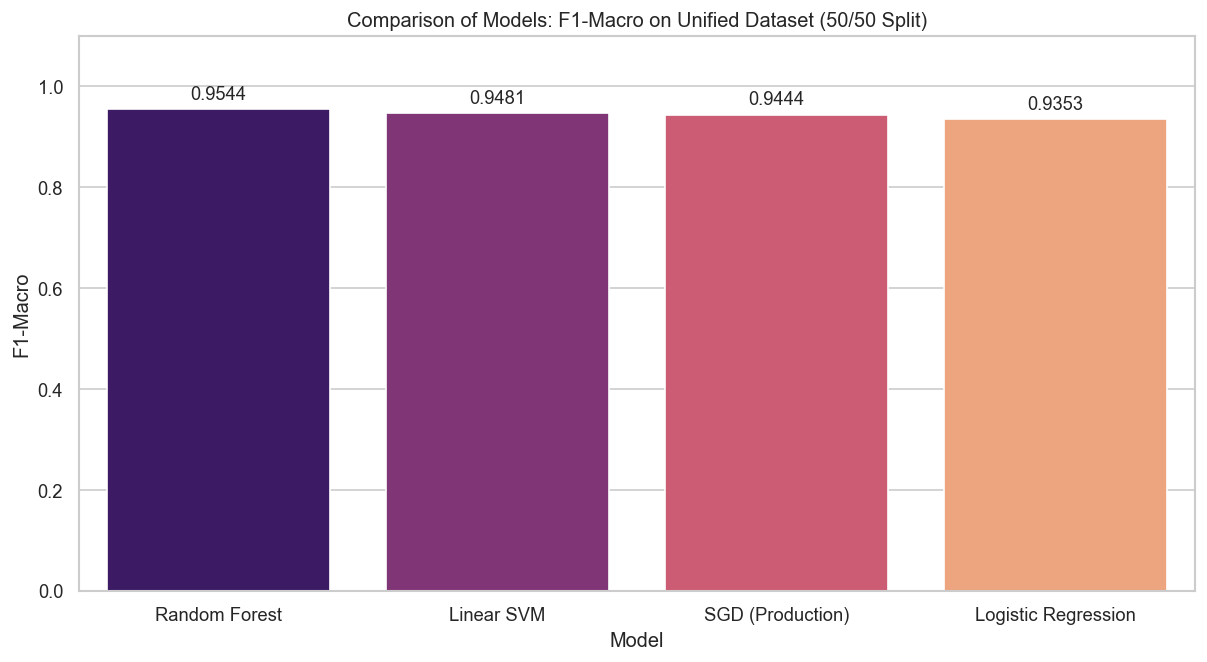
\includegraphics[width=0.8\textwidth]{figures/comparation_models.png}
    \caption{Resultados de la comparativa con el dataset conjunto}
    \label{fig:comparation_models}
\end{figure}

Tras las pruebas, el modelo \textbf{Linear SVM} obtuvo un \textbf{F1-Macro de 0.9481} con el dataset unificado \ref{fig:comparation_models} y \textbf{F1-Macro de 1} con el dataset modificado y revisado, superando al SGD original. Este modelo ofrece el mejor equilibrio entre:
\begin{enumerate}
    \item \textbf{Precisión}: Máxima eficacia en la separación de categorías complejas (como ``Ocio'' vs ``Ocio, Vacaciones'').
    \item \textbf{Explicabilidad}: Al ser un modelo lineal, permite auditar los pesos de las palabras clave.
    \item \textbf{Eficiencia}: Mantiene una huella de memoria ligera y tiempos de inferencia casi instantáneos.
\end{enumerate}




Por tanto, se ha seleccionado \texttt{LinearSVM.joblib} como el modelo principal para la implementación en el sistema de producción.


\newpage
\section{Conclusiones}
\label{sec:conclusiones}

El desarrollo de este sistema demuestra que modelos lineales clásicos como el \textbf{Linear SVM}, combinados con una vectorización TF-IDF bien configurada, son extremadamente competitivos para tareas de clasificación de texto financiero corto. 

La unión de los datasets original y modificado ha sido clave para mejorar la robustez ante diferentes estilos de redacción. La adopción final del modelo SVM garantiza que el sistema no solo sea preciso, sino también transparente y eficiente para su despliegue real. Como líneas futuras, se podría explorar el ajuste fino de hiperparámetros (\textit{Hyperparameter Tuning}) para arañar los últimos puntos de precisión en las categorías combinadas.


\newpage
\printbibliography[title={Referencias Bibliográficas}]


\end{document}
